% This is "sig-alternate.tex" V2.1 April 2013
% This file should be compiled with V2.5 of "sig-alternate.cls" May 2012
%
% This example file demonstrates the use of the 'sig-alternate.cls'
% V2.5 LaTeX2e document class file. It is for those submitting
% articles to ACM Conference Proceedings WHO DO NOT WISH TO
% STRICTLY ADHERE TO THE SIGS (PUBS-BOARD-ENDORSED) STYLE.
% The 'sig-alternate.cls' file will produce a similar-looking,
% albeit, 'tighter' paper resulting in, invariably, fewer pages.
%
% ----------------------------------------------------------------------------------------------------------------
% This .tex file (and associated .cls V2.5) produces:
%       1) The Permission Statement
%       2) The Conference (location) Info information
%       3) The Copyright Line with ACM data
%       4) NO page numbers
%
% as against the acm_proc_article-sp.cls file which
% DOES NOT produce 1) thru' 3) above.
%
% Using 'sig-alternate.cls' you have control, however, from within
% the source .tex file, over both the CopyrightYear
% (defaulted to 200X) and the ACM Copyright Data
% (defaulted to X-XXXXX-XX-X/XX/XX).
% e.g.
% \CopyrightYear{2007} will cause 2007 to appear in the copyright line.
% \crdata{0-12345-67-8/90/12} will cause 0-12345-67-8/90/12 to appear in the copyright line.
%
% ---------------------------------------------------------------------------------------------------------------
% This .tex source is an example which *does* use
% the .bib file (from which the .bbl file % is produced).
% REMEMBER HOWEVER: After having produced the .bbl file,
% and prior to final submission, you *NEED* to 'insert'
% your .bbl file into your source .tex file so as to provide
% ONE 'self-contained' source file.
%
% ================= IF YOU HAVE QUESTIONS =======================
% Questions regarding the SIGS styles, SIGS policies and
% procedures, Conferences etc. should be sent to
% Adrienne Griscti (griscti@acm.org)
%
% Technical questions _only_ to
% Gerald Murray (murray@hq.acm.org)
% ===============================================================
%
% For tracking purposes - this is V2.0 - May 2012

\documentclass{sig-alternate-05-2015}
\usepackage{placeins}
\usepackage{epstopdf}


\begin{document}

% Copyright
%\setcopyright{acmcopyright}
%\setcopyright{acmlicensed}
%\setcopyright{rightsretained}
%\setcopyright{usgov}
%\setcopyright{usgovmixed}
%\setcopyright{cagov}
%\setcopyright{cagovmixed}


%
% --- Author Metadata here ---
%\conferenceinfo{WOODSTOCK}{'97 El Paso, Texas USA}
%\CopyrightYear{2007} % Allows default copyright year (20XX) to be over-ridden - IF NEED BE.
%\crdata{0-12345-67-8/90/01}  % Allows default copyright data (0-89791-88-6/97/05) to be over-ridden - IF NEED BE.
% --- End of Author Metadata ---

\title{Recommendation Algorithms for User First Booking on Airbnb}
%
% You need the command \numberofauthors to handle the 'placement
% and alignment' of the authors beneath the title.
%
% For aesthetic reasons, we recommend 'three authors at a time'
% i.e. three 'name/affiliation blocks' be placed beneath the title.
%
% NOTE: You are NOT restricted in how many 'rows' of
% "name/affiliations" may appear. We just ask that you restrict
% the number of 'columns' to three.
%
% Because of the available 'opening page real-estate'
% we ask you to refrain from putting more than six authors
% (two rows with three columns) beneath the article title.
% More than six makes the first-page appear very cluttered indeed.
%
% Use the \alignauthor commands to handle the names
% and affiliations for an 'aesthetic maximum' of six authors.
% Add names, affiliations, addresses for
% the seventh etc. author(s) as the argument for the
% \additionalauthors command.
% These 'additional authors' will be output/set for you
% without further effort on your part as the last section in
% the body of your article BEFORE References or any Appendices.

\numberofauthors{3} %  in this sample file, there are a *total*
% of EIGHT authors. SIX appear on the 'first-page' (for formatting
% reasons) and the remaining two appear in the \additionalauthors section.
%
\author{
% You can go ahead and credit any number of authors here,
% e.g. one 'row of three' or two rows (consisting of one row of three
% and a second row of one, two or three).
%
% The command \alignauthor (no curly braces needed) should
% precede each author name, affiliation/snail-mail address and
% e-mail address. Additionally, tag each line of
% affiliation/address with \affaddr, and tag the
% e-mail address with \email.
%
% 1st. author
\alignauthor Zhao Wang \\
       \affaddr{Northeastern University}\\
       \affaddr{Seattle, WA}\\
       \email{\large wang.zhao2@husky.neu.edu}
% 2nd. author
\alignauthor Zerui Ma \\
      \affaddr{Northeastern University}\\
       \affaddr{Seattle, WA}\\
       \email{\large zeruima1989@gmail.com}
% 3rd. author
\alignauthor Heng Xu\\
       \affaddr{Northeastern University}\\
       \affaddr{Seattle, WA}\\
       \email{\large xu.he@husky.neu.edu}
}
% There's nothing stopping you putting the seventh, eighth, etc.
% author on the opening page (as the 'third row') but we ask,
% for aesthetic reasons that you place these 'additional authors'
% in the \additional authors block, viz.

% Just remember to make sure that the TOTAL number of authors
% is the number that will appear on the first page PLUS the
% number that will appear in the \additionalauthors section.

\maketitle
\begin{abstract}
Airbnb has become more and more popular under the trend of sharing economy. In order to attract new users to place their first booking on Airbnb and offer a more personalized experience, we aim to build a recommendation system by using collaborative filtering approach, to predict which country these new users will make their first booking. Also the hosting data for various countries will be analyzed to provide better insight around booking area.
\end{abstract}


%
% The code below should be generated by the tool at
% http://dl.acm.org/ccs.cfm
% Please copy and paste the code instead of the example below. 
%
\begin{CCSXML}
<ccs2012>
 <concept>
  <concept_id>10010520.10010553.10010562</concept_id>
  <concept_desc>Computer systems organization~Embedded systems</concept_desc>
  <concept_significance>500</concept_significance>
 </concept>
 <concept>
  <concept_id>10010520.10010575.10010755</concept_id>
  <concept_desc>Computer systems organization~Redundancy</concept_desc>
  <concept_significance>300</concept_significance>
 </concept>
 <concept>
  <concept_id>10010520.10010553.10010554</concept_id>
  <concept_desc>Computer systems organization~Robotics</concept_desc>
  <concept_significance>100</concept_significance>
 </concept>
 <concept>
  <concept_id>10003033.10003083.10003095</concept_id>
  <concept_desc>Networks~Network reliability</concept_desc>
  <concept_significance>100</concept_significance>
 </concept>
</ccs2012>  
\end{CCSXML}



%
% End generated code
%

%
%  Use this command to print the description
%
\printccsdesc

% We no longer use \terms command
%\terms{Theory}

\keywords{Learning Algorithms; Recommendation Systems; Collaborative Filtering; Cluster Models}

\section{Introduction}
Data mining is the process of discovering interesting patterns from massive amounts of data. As a knowledge discovery process, it typically involves data cleaning, data integration, data selection, data transformation, pattern discovery, pattern evaluation, and knowledge presentation\cite{data mining}. The science of learning plays a key role in the fields of data mining, statistics and artificial intelligence, intersecting with areas of engineering and other disciplines\cite{statistical}.  In a typical scenario, a quantitative or categorical outcome measurement is predicted based on a set of features.

Recommendation algorithms are a kind of learning algorithms which are widely used on e-commerce web sites.  they use input about a customer\'s interests to generate a list of recommended items. Most recommendation algorithms are designed for finding similar customers, where they aggregate items from the similar customers, eliminates items the user has already purchased or rated, and recommends the remaining items to the user. The popular versions of these algorithms are collaborative filtering and cluster models. In the collaborative filtering, the similarity of customers is measured by the cosine of the angle between the two vectors which represent users' interests\cite{analysis}. Using this algorithm to generate recommendations is computationally expensive, but it can be released by dimensionally reduction techniques\cite{collaborative}. To find the similar customers to the user, cluster models divide the customer base into many segments and treat the task as a classification problem\cite{clustering}.  Some algorithms classify users into multiple segments and describe the strength of each relationship\cite{cf}. Besides grouping the user to the similar customers, other algorithms such as search-based methods and item-to-item collaborative filtering focus on finding similar items\cite{item2item}. Search- or content-based methods treat the recommendations problem as a search for related items\cite{massive}.

User experience is now a critical factor to keep users and attract new users among web applications. That is the reason Airbnb wants to provide personalized and unique experience for its new users, thus Airbnb need an effective recommendation system to recommend a country for first-time booking.

However, the main challenge here is that Airbnb doesn't have the travel history or other type of the traveling data of new users, the only data available here is basic feature such as age, gender, session log etc., basically like a white paper to a recommendation system. While a typical recommendation system might make recommendation based on a few strongly related features, the system designed here need to focus on correctly classify similar users first, then trying to make recommendation with some relatively strong features. And that is why we choose collaborative filtering as our first-step approach.

\section{Dataset Description}
In this section, the data sets which are applied for the recommendation are introduced. The data is  consisted of two parts: the first one is the list of users\' first booking destinations as well as their demographics and web session records; the other is the aggregated public host information dataset which is sourced from publicly available information from the Airbnb site. By analyzing the statistics of the source data, we can have an overview of the entire data and help to decide how to apply for the recommendation algorithms.

\subsection{User data set}
In the list of user first booking, each user is specified by a unique string id and each instance contains multiple types of properties for that user, which should be date, numerical, categorical, etc. There exists missing values in each fields, which should be handled before building recommendation model. The users whose destination countries are unavailable (indicated as NDF) are also need to be filtered out. The details of user properties are described as Table.\ref{table:users}.

\begin{table}[!htb]
\caption{User Data Statistics}
\label{table:users}
\begin{tabular}{|c|c|l|} \hline
field & type & description  \\ \hline                                                                                                                              
id & string & unique for each user \\ \hline                                                                                                                     
\shortstack{date\_account\\ \_created} & date & ~ \\ \hline                                                                                                                                             
\shortstack{timestamp\_first\\ \_active}  & timestampe & ~  \\ \hline                                                                                                                                          \shortstack{date\_first\\ \_booking} & date & ~ \\ \hline                                                                                                                                             
gender & categorical & \shortstack[l]{FEMALE, MALE, \\OTHER, unknown} \\ \hline                                                                                                                 
age & numerical & 1 to 150  \\ \hline                                                                                                                      
signup\_method  & categorical & basic, facebook, google  \\ \hline                                                                                                                       
signup\_flow & numerical & 0 to 25  \\ \hline                                                                                                                                  language & categorical & en, zh, fr, es, ko, de, etc.  \\ \hline                                                                                                              
affiliate\_channel  & categorical & \shortstack[l]{api, content, direct, etc}  \\ \hline
affiliate\_provider  & categorical & \shortstack[l]{bing, facebook, google, etc} \\ \hline
\shortstack{first\_affiliate\\ \_tracked} & categorical & \shortstack[l]{linked, local ops, \\ product, etc.} \\ \hline
signup\_app & categorical & Android, iOS, Moweb, Web \\ \hline
first\_device\_type & categorical & \shortstack[l]{Android Phone, iPad, \\ iPhone, Mac Desktop, etc.} \\ \hline
first\_browser  & categorical & \shortstack[l]{Chrome, Safari, Firefox, etc.} \\ 
\hline \end{tabular}
\end{table}

Since most records in the dataset have no first booking destination, we only focus on the instances with available destination. After filtering the records without specific destinations, the numbers of the users for each country are as Table.\ref{table:destination} described. The most number of remaining users is for other destinations, which is less useful for the recommendation. The instances with specific destinations are the data we can use to build the predication model for new users.

\begin{table}[!htb]
\centering
\caption{Users First Booking Destination}
\label{table:destination}
\begin{tabular}{|c|c|l|} \hline
Destination Country & Population\\ \hline
AU & 537 \\ \hline
CA & 1425 \\ \hline
DE & 1059 \\ \hline
ES & 2243 \\ \hline
FR & 5013 \\ \hline
GB & 2318 \\ \hline
IT & 2827 \\ \hline
NL & 757 \\ \hline
PT & 217 \\ \hline
US &  62263 \\ \hline
other & 10075 \\
\hline\end{tabular}
\end{table}

\begin{figure}
\centering
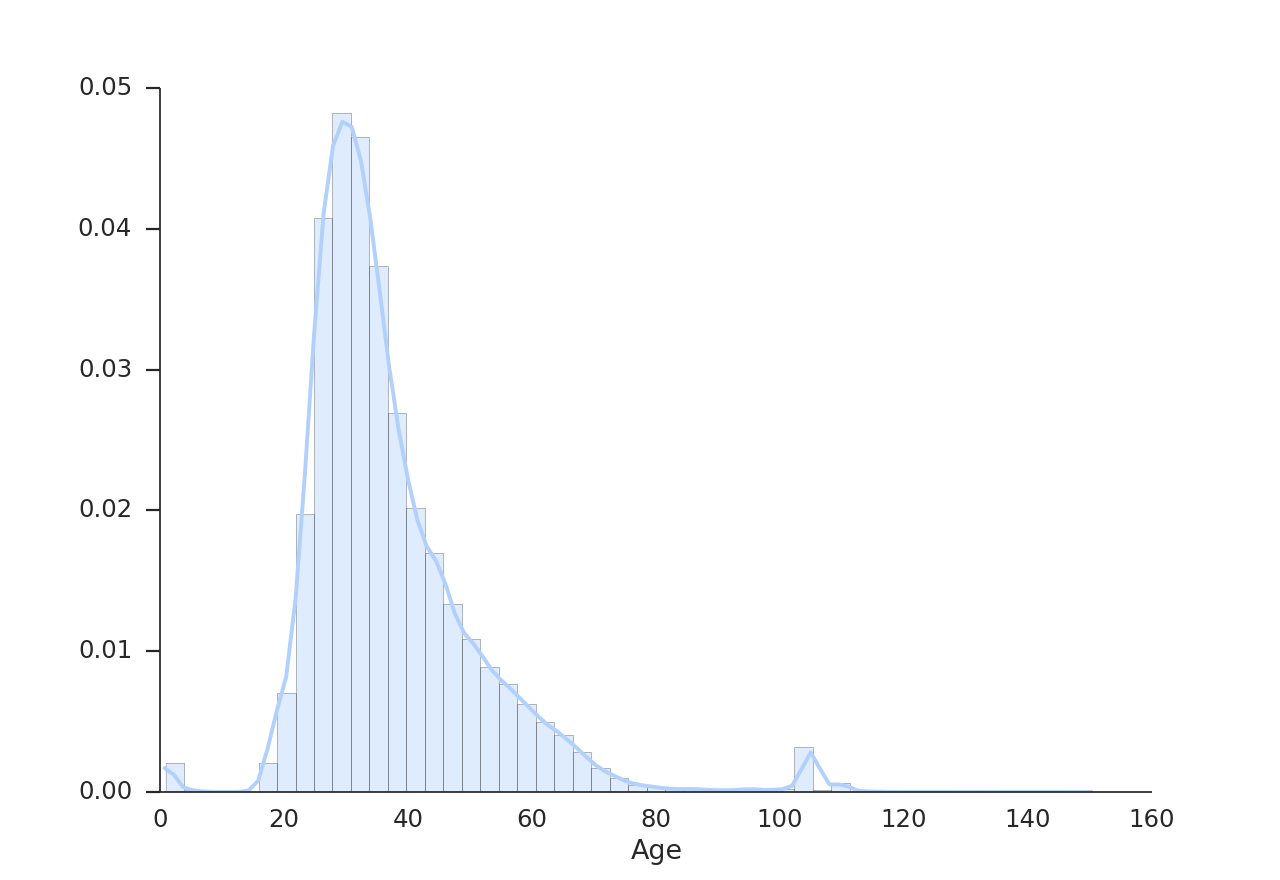
\includegraphics[height=2in, width=3in]{AgeDistribution}
\caption{Age Distribution for Users on Airbnb}
\label{fig:age distribution}
\end{figure}

\FloatBarrier
\subsection{Hosts data set}
The other data set is about detailed information of host listings among 16 countries available on Airbnb, although it covers almost all the countries in new user data set, but PT(Portugal) listing data is missing here.

This listing data set contains most of the public information available on Airbnb, and lots of features such as listing price, listing rating score, host registration information and neighbourhood etc., may help recommendation system identify better listings among target country for new users. However, due to the limitation of new user data, the recommendation on this part is most likely to be based on features weighted by common sense: highest rated, best available price etc..

\begin{figure}
\centering
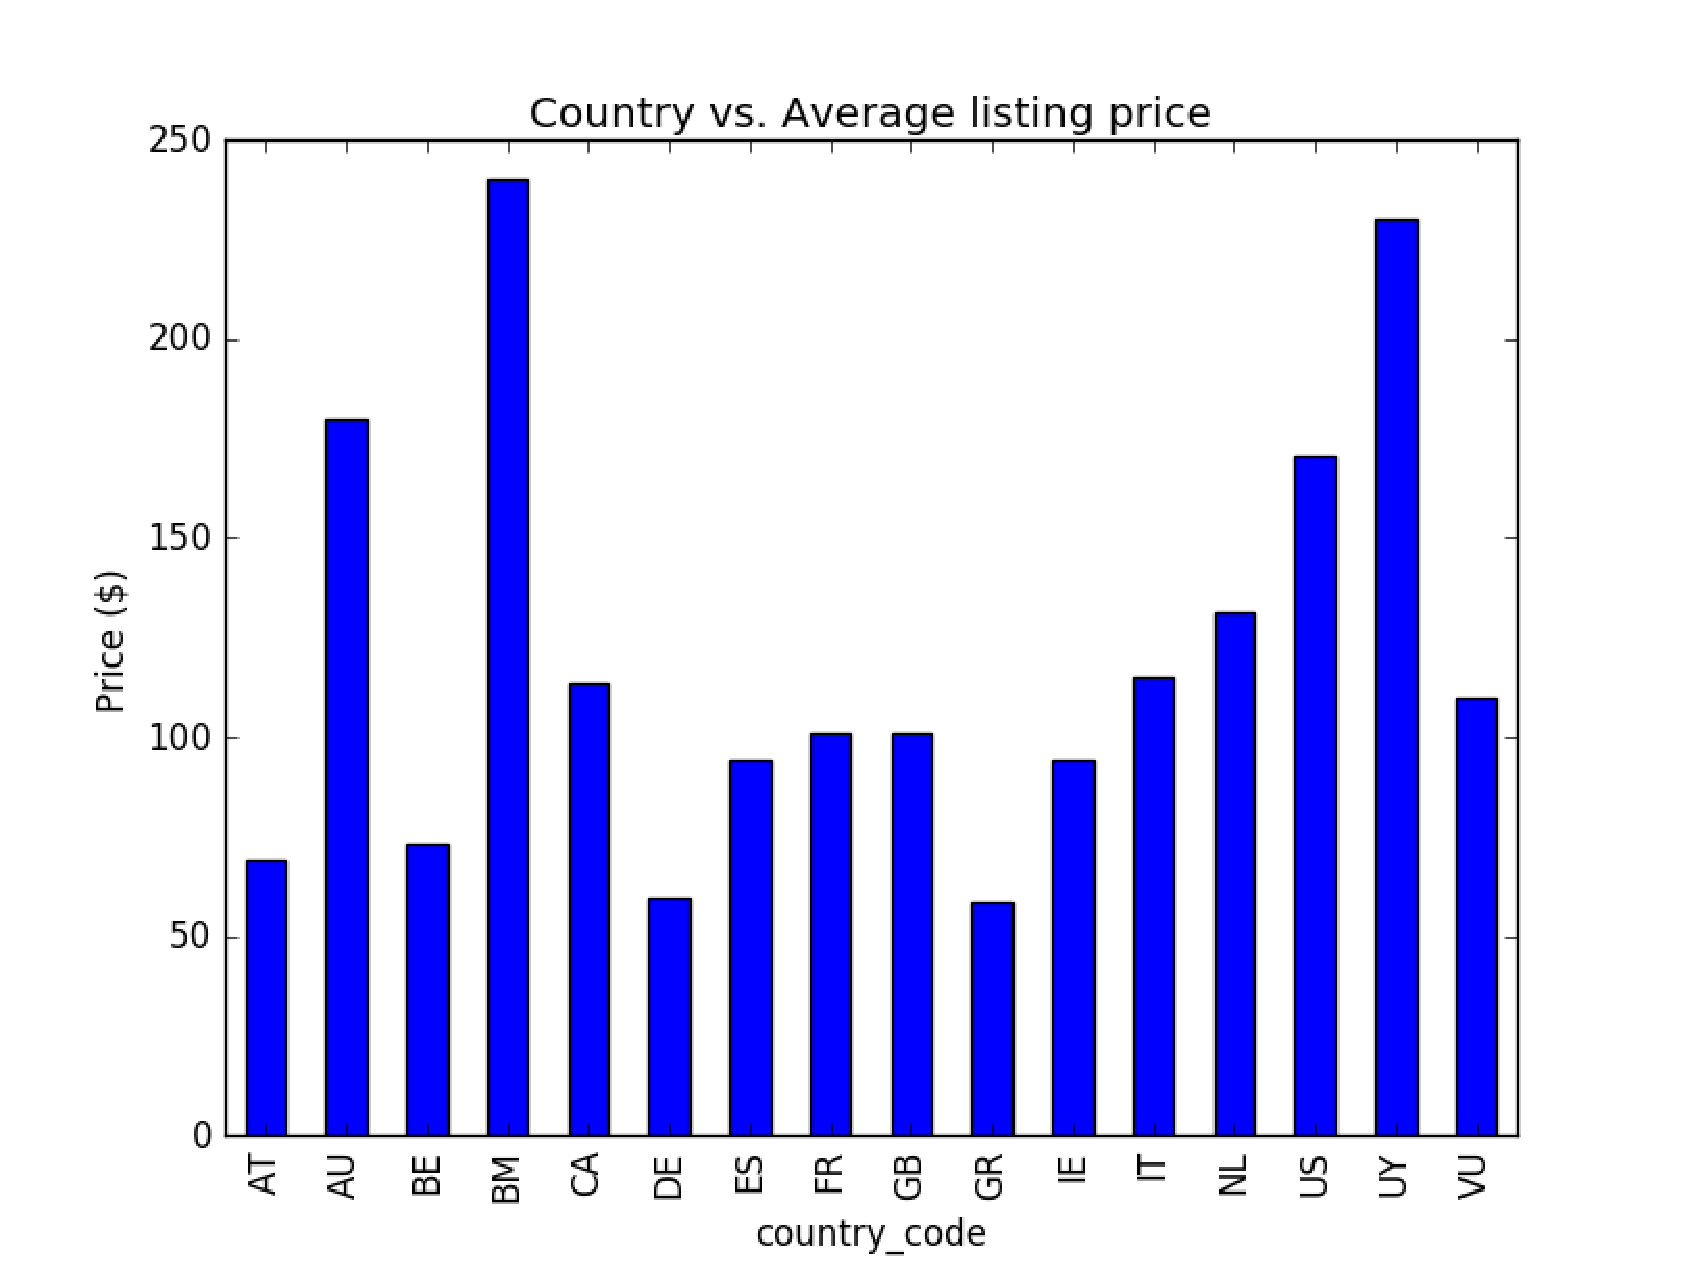
\includegraphics[height=2in, width=3in]{country-avgPrice}
\caption{Average price distribution among countries}
\end{figure}

Since listing price is showed in dollar, so the average listing price distribution is influenced by currency exchange rate in some extent, but besides that fact, the average listing price definitely reflects the popularity of these destination countries. BM(Bermuda) is a typical high-end vacation hot spot, but it's surprised to see UY(Uruguay) has such a high average price, maybe because the retrived UY listings is very limited. Other than these two countries, AU and US are the most expensive countries to go on Airbnb. It's interesting to see AU has higher average listing price over US, a possible explaination for this could be the number of listings in US is much greater than AU's, thus competetion over the host has lowered the average listing price in US.

\begin{figure}
\centering
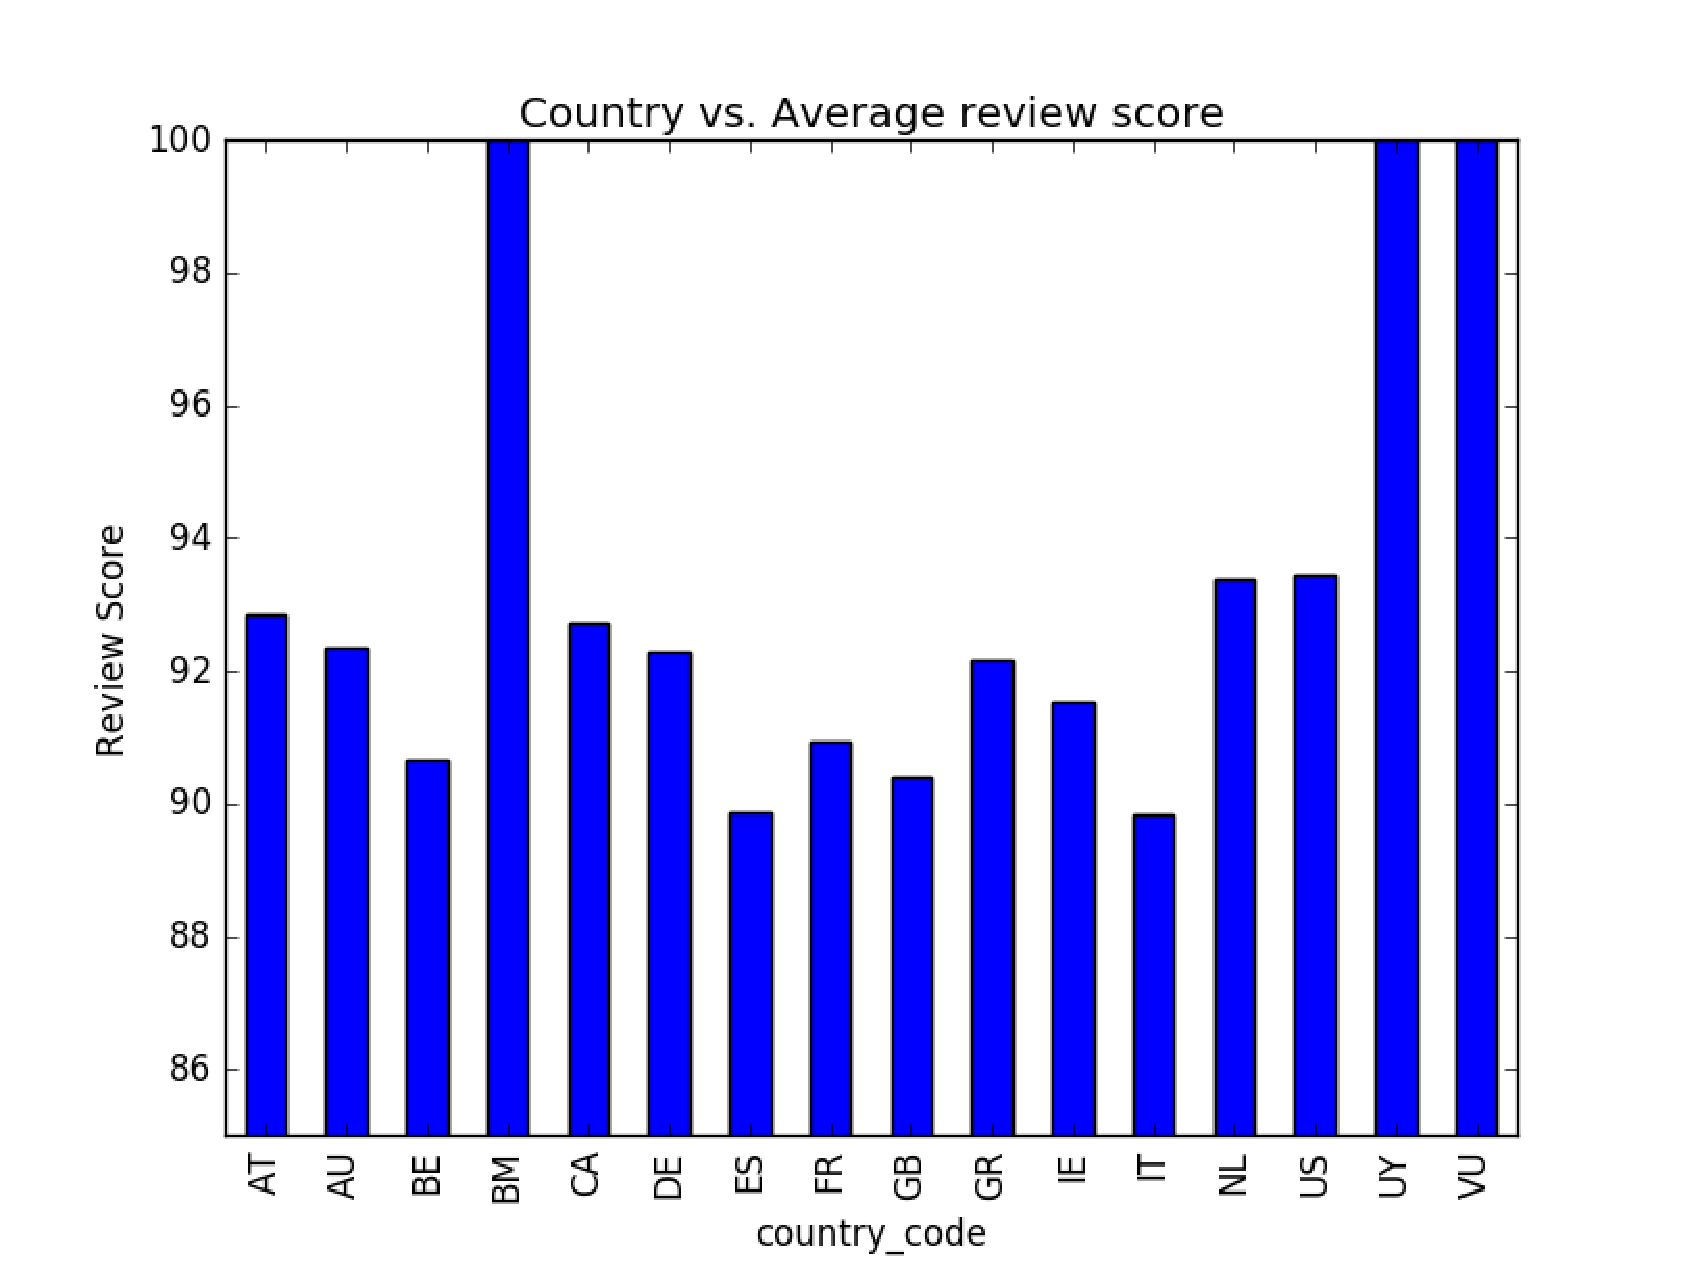
\includegraphics[height=2in, width=3in]{country-avgRating}
\caption{Average rating score distribution among countries}
\end{figure}

When comes to average review scores, most of countries get over score of 90. BM, UY and VU receives average score of 100, but since the number of listing of these 3 countries in this data set is very limited, it probably has large bias here. Besides these 3 countries, US and NL is probably best reviewed place to go on Airbnb, IT and ES is the worst reviewed, but still has average score of over 89.

\FloatBarrier
\section{Proposed Algorithmic Approach}
Using collaborative filtering to aggregate the similar users based on their first booking on Airbnb. The similarity between users is measured by cosine of the angle between the two vectors which indicate user properties. Dimensionality reduction should be applied to reduce computational complexity and speed up the algorithm.

\subsection{Data preprocess}
Since each 


\begin{table}[!htb]
\centering
\caption{Data Preprocess}
\label{table:preprocess}
\begin{tabular}{|c|l|} \hline
Processed Attribute & Description\\ \hline
\shortstack{Lag between date\_first\_booking \\ and date\_account\_created} & 
\shortstack[l]{Divided into 4 categories\: \\ =0, <0, >0, NA.}\\ \hline
\shortstack{Lag between date\_first\_booking \\ and timestamp\_first\_active} & 
\shortstack[l]{Divided into 3 categories\: \\ =0, >0, NA}\\ \hline
Age & 
\shortstack[l]{Replace the missing values \\
with the conditional mean; \\
scale the age with mean \\
and standard variance} \\ \hline
Others & Original value \\
\hline\end{tabular}
\end{table}


\subsection{Basic and Ensemble Classifiers}

\begin{figure}
\centering
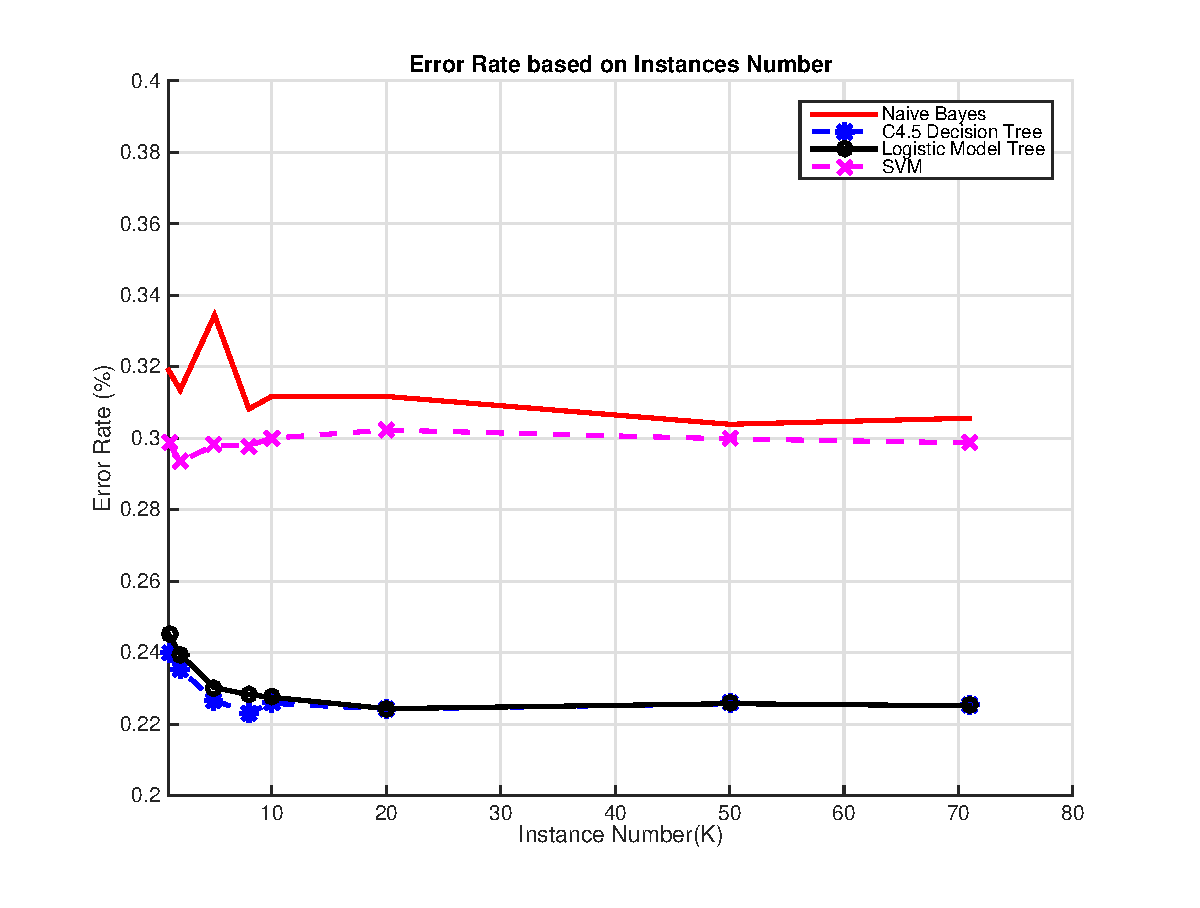
\includegraphics[height=2in, width=3in]{Basic_Classifiers}
\caption{Error Rates for Basic Classifier}
\label{fig:basic classifier}
\end{figure}

\begin{figure}
\centering
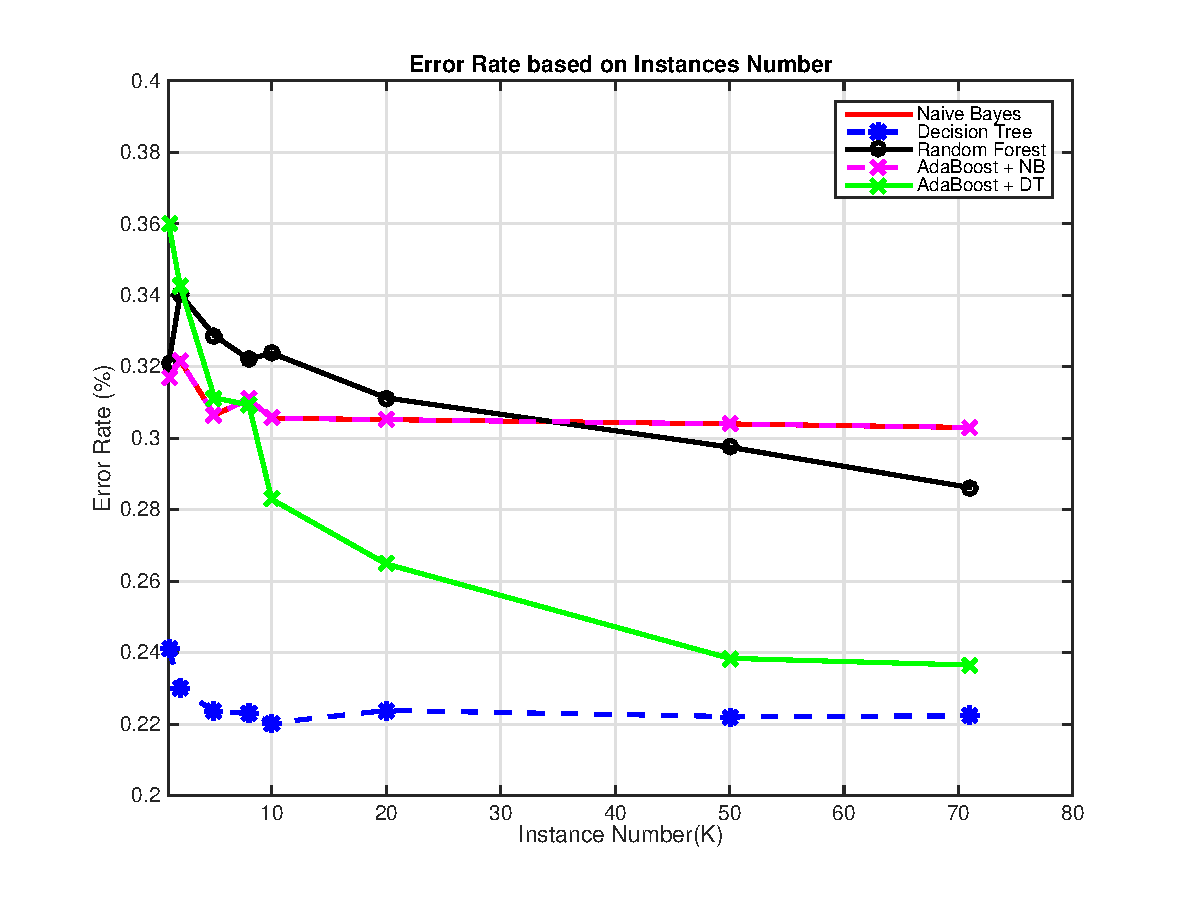
\includegraphics[height=2in, width=3in]{Ensemble_Classifiers}
\caption{Error Rates for Ensemble Classifier}
\label{fig:ensemble classifier}
\end{figure}

\begin{figure}
\centering
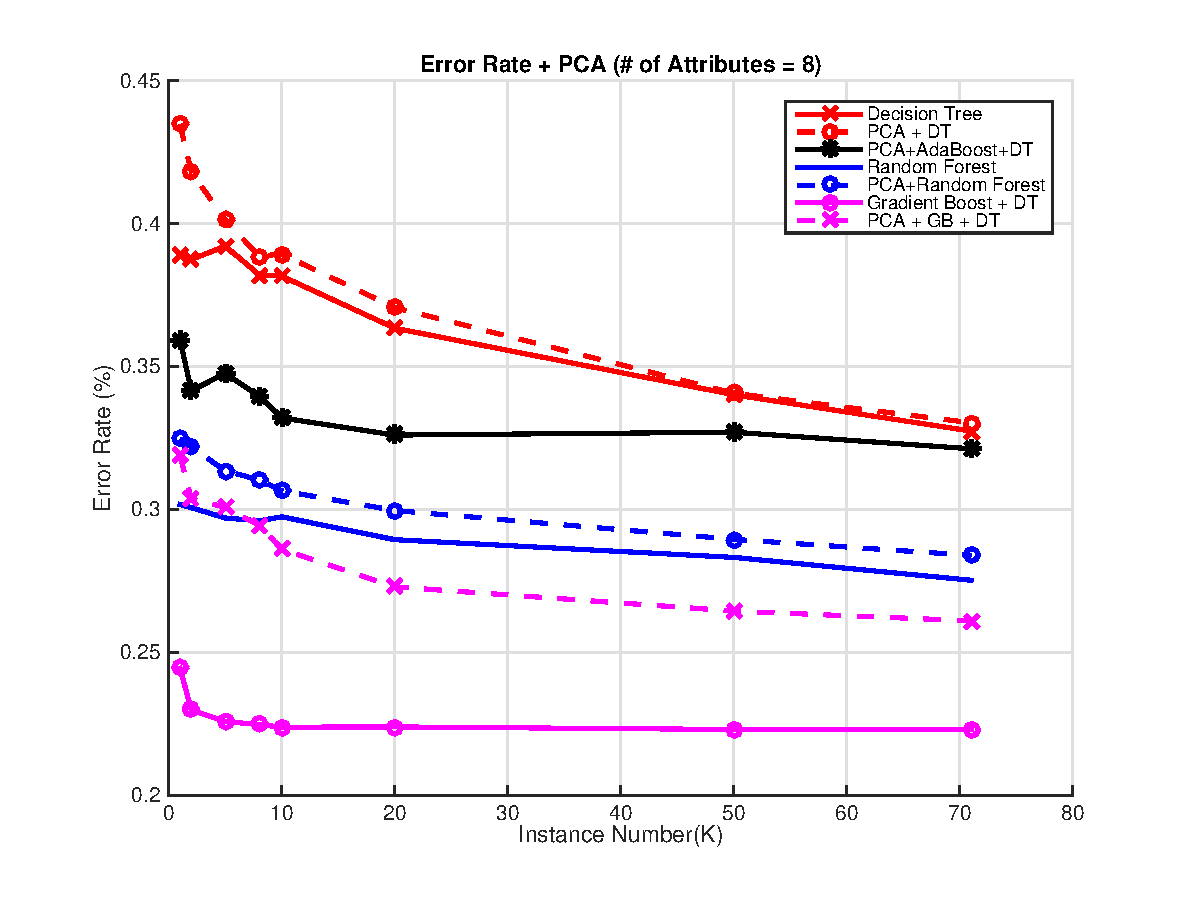
\includegraphics[height=2in,width=3in]{PCA_Classifiers}
\caption{PCA with Classifiers}
\label{fig:pca}
\end{figure}

\subsection{Collaborative Filtering}

\begin{table}[!htb]
\centering
\caption{Clustering Parameters}
\label{table:clustering}
\begin{tabular}{|c|c|c|c|} \hline
\shortstack[l]{Percentage Change \\ of WGSS} & Cluster Num & WGSS & Error Rate \\ \hline
< 0.3\% & 10 & 114013 & 0.3036 \\ \hline
< 0.1\% & 17 & 106895 & 0.2978 \\ \hline
< 0.03\% & 67 & 84909 & 0.2700 \\ \hline
< 0.003\% & 163 & 73112 & 0.2330 \\ \hline
< 0.001\% & 424 & 55412 & 0.2137 \\
\hline\end{tabular}
\end{table}

\begin{figure}
\centering
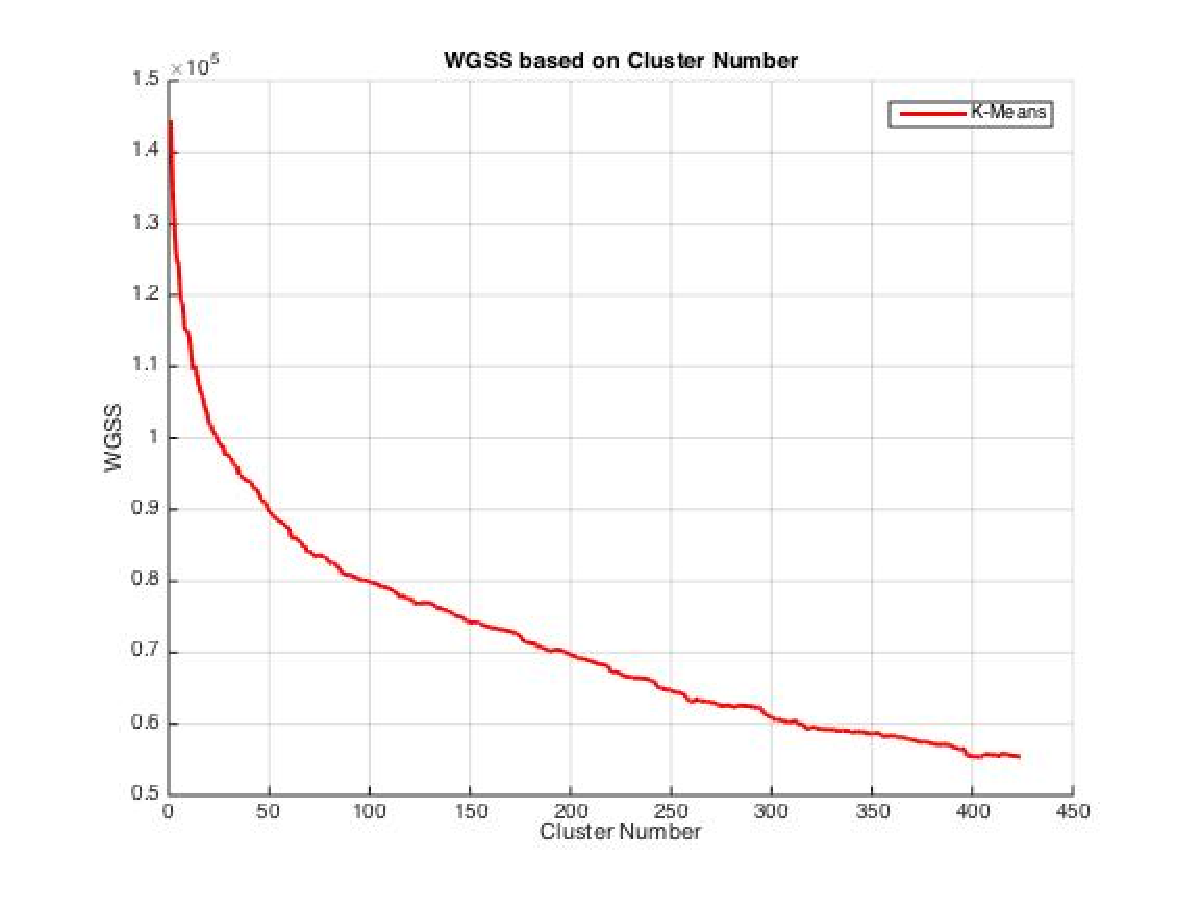
\includegraphics[height=2in,width=3in]{K_Means}
\caption{WGSS based on Clusters}
\label{fig:k means}
\end{figure}

\section{Conclusion}

\medskip

\begin{thebibliography}{9}
\bibitem{data mining} Han, J., Kamber, M., and Pei, J. , "Data Mining: Concepts and Techniques", 3rd Edition, 2011.
\bibitem{statistical} Hastie T., Tibshirani R., and Friedman, J. , "The Elements of Statistical Learning: Data Mining, Inference, and Prediction", 2nd Edition, 2009.
\bibitem{analysis} B.M. Sarwarm et al., "Analysis of Recommendation Algorithms for E-Commerce", ACM Conf. Electronic Commerce, ACM Press, 2000, pp.158-167.
\bibitem{collaborative} K. Goldberg et al., "Eigentaste: A Constant Time Collaborative Filtering Algorithm", Information Retrieval J., vol. 4, no. 2, July 2001, pp. 133-151.
\bibitem{clustering} P.S. Bradley, U.M. Fayyad, and C. Reina, "Scaling Clustering Algorithms to Large Databases", Knowledge Discovery and Data Mining, Kluwer Academic, 1998, pp. 9-15.
\bibitem{cf} L. Ungar and D. Foster, "Clustering Methods for Collaborative Filtering", Proc. Workshop on Recommendation Systems, AAAI Press, 1998.
\bibitem{item2item} G. Linden, B. Smith, and J. York, "Amazon.com recommendations: item-to-item collaborative filtering", Internet Computing 7:1, 2003, pp. 76-80.
\bibitem{massive} Leskovec, J., Rajaraman, A., and Ullman, "Mining of Massive Datasets", 2nd Edition, 2004, pp. 307-341.

\end{thebibliography}
%\balancecolumns % GM June 2007
% That's all folks!
\end{document}
